\section{SRResCGAN实验}

\begin{frame}{训练结果}
    第一次训练, $lr_{G}=0.0001, lr_{D}=0.0003$最终的D\_fake\_output和D\_real\_output一直相差较大, 说明判别器远强于生成器; 增大生成器学习率$lr_{G}=0.001$, 依然如此. 除学习率外, 可调整参数有网络结构, 各种损失函数的权重和类型. 
\end{frame}

\begin{frame}{PNSR SSIM}
    \footnotesize
    \begin{tabular}{l|p{3cm}|p{3cm}}
        \hline
                 & PNSR & SSIM     \\ \hline
        01Bicubic & 17.89dB & 0.3750 \\ \hline
        01SRResCGAN & 19.45dB & 0.4412 \\ \hline
        02BIcubic &  19.48dB & 0.4240 \\ \hline
        02SRResCGAN & 21.34dB & 0.4930 \\ \hline
        03BIcubic &  23.83dB & 0.6836 \\ \hline
        03SRResCGAN & 24.30dB & 0.6845 \\ \hline
        04BIcubic &  18.54dB & 0.3384 \\ \hline
        04SRResCGAN & 19.15dB & 0.3536 \\ \hline
        05BIcubic &  21.42dB & 0.4730 \\ \hline
        05SRResCGAN & 22.56dB & 0.4893 \\ \hline
    \end{tabular}

    一方面没有训练好; 一方面本身影像对存在一定差异
\end{frame}

\begin{frame}{细节对比}
    \begin{figure}[!htbp]
        \centering
        \subfloat[gt]{\label{fig:0301a}
        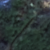
\includegraphics[height=1cm]{pic/pic0301gt.png}}
        \quad
        \subfloat[bic]{\label{fig:0301b}
        
\includegraphics[height=1cm]{pic/pic0301bic.png}}
        \quad
        \subfloat[sr]{\label{fig:0301c}
        
\includegraphics[height=1cm]{pic/pic0301sr.png}}
        \caption{细部对比01}
        \label{fig:0301}
    \end{figure}

    \begin{figure}[!htbp]
        \centering
        \subfloat[gt]{\label{fig:0302a}
        
\includegraphics[height=1cm]{pic/pic0302gt.png}}
        \quad
        \subfloat[bic]{\label{fig:0302b}
        
\includegraphics[height=1cm]{pic/pic0302bic.png}}
        \quad
        \subfloat[sr]{\label{fig:0302c}
        
\includegraphics[height=1cm]{pic/pic0302sr.png}}
        \caption{细部对比02}
        \label{fig:0302}
    \end{figure}

    
\end{frame}

\begin{frame}{细节对比}
    \begin{figure}[!htbp]
        \centering
        \subfloat[gt]{\label{fig:0303a}
        
\includegraphics[height=1cm]{pic/pic0303gt.png}}
        \quad
        \subfloat[bic]{\label{fig:0303b}
        
\includegraphics[height=1cm]{pic/pic0303bic.png}}
        \quad
        \subfloat[sr]{\label{fig:0303c}
        
\includegraphics[height=1cm]{pic/pic0303sr.png}}
        \caption{细部对比03}
        \label{fig:0303}
    \end{figure}

    \begin{figure}[!htbp]
        \centering
        \subfloat[gt]{\label{fig:0304a}
        
\includegraphics[height=1cm]{pic/pic0304gt.png}}
        \quad
        \subfloat[bic]{\label{fig:0304b}
        
\includegraphics[height=1cm]{pic/pic0304bic.png}}
        \quad
        \subfloat[sr]{\label{fig:0304c}
        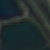
\includegraphics[height=1cm]{pic/pic0304sr.png}}
        \caption{细部对比04}
        \label{fig:0304}
    \end{figure}
\end{frame}

\begin{frame}{细节对比}
    \begin{figure}[!htbp]
        \centering
        \subfloat[gt]{\label{fig:0305a}
        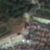
\includegraphics[height=1cm]{pic/pic0305gt.png}}
        \quad
        \subfloat[bic]{\label{fig:0305b}
        
\includegraphics[height=1cm]{pic/pic0305bic.png}}
        \quad
        \subfloat[sr]{\label{fig:0305c}
        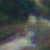
\includegraphics[height=1cm]{pic/pic0305sr.png}}
        \caption{细部对比05}
        \label{fig:0305}
    \end{figure}

    \begin{figure}[!htbp]
        \centering
        \subfloat[gt]{\label{fig:0306a}
        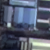
\includegraphics[height=1cm]{pic/pic0306gt.png}}
        \quad
        \subfloat[bic]{\label{fig:0306b}
        
\includegraphics[height=1cm]{pic/pic0306bic.png}}
        \quad
        \subfloat[sr]{\label{fig:0306c}
        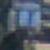
\includegraphics[height=1cm]{pic/pic0306sr.png}}
        \caption{细部对比06}
        \label{fig:0306}
    \end{figure}
\end{frame}